\documentclass[aspectratio=1610]{beamer}

\usepackage{transparent}

\usetheme{Copenhagen}

\title[Student Engineer Design Portfolio]{Design Portfolio}
\subtitle{ESC102 Praxis II}
\author[Page \insertframenumber]{Kevin (Zerui) Wang}
\institute{University of Toronto}
\date{\today}

\begin{document}
{
\setbeamertemplate{footline}{}
\begin{frame}
\titlepage
\end{frame}
}
\addtocounter{framenumber}{-1}

{
% \setbeamertemplate{background}{
%     
\includegraphics[width=\paperwidth,height=\paperheight]{images/portfolio.jpg}
% }
\begin{frame}{Table of Contents}
    \tableofcontents
\end{frame}
}

\section{Egineering, Design, and Engineering Design}

\begin{frame}{Table of Contents}
\end{frame}
\section{Position in Context}
\begin{frame}{Table of Contents}
\end{frame}
\subsection{Values}
\begin{frame}{Table of Contents}
\end{frame}
\subsection{Abilities}
\begin{frame}{Table of Contents}
\end{frame}
\subsection{Strengths}
\begin{frame}{Table of Contents}
\end{frame}
\subsection{Biases}
\subsection{Areas for Improvement}
\section{Design Experiences}
\subsection{Praxis I}
\subsection{CIV102 Bridge}
\subsection{Praxis II}

{
% \setbeamertemplate{background}{
%     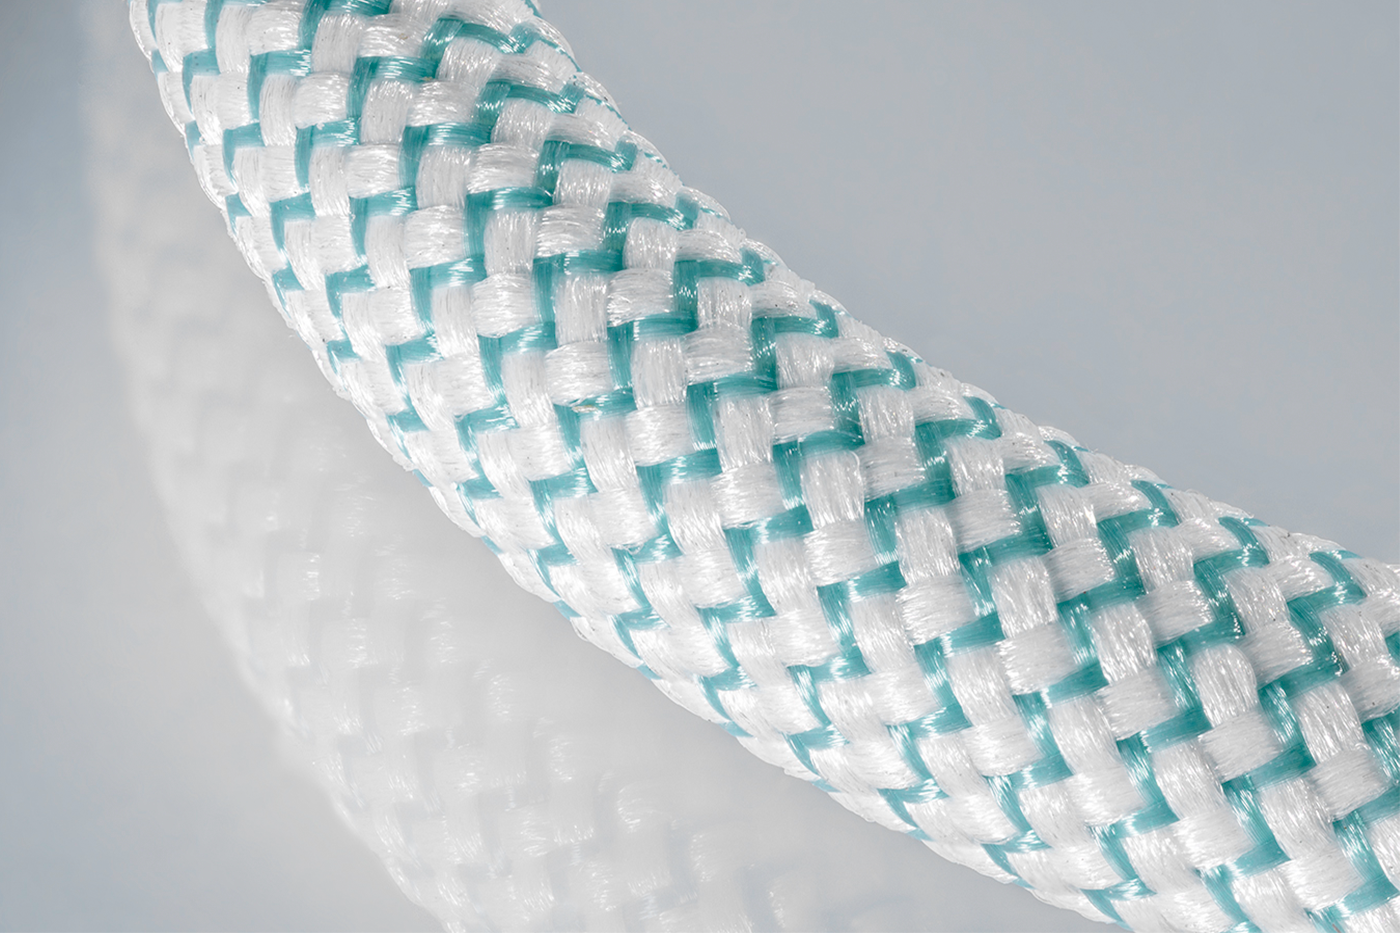
\includegraphics[width=\paperwidth,height=\paperheight]{images/braid.png}
% }
\begin{frame}{Table of Contents}
\end{frame}
}

\begin{frame}
    \frametitle{Title}
    lorem dolor sit amet
\end{frame}

\begin{frame}
    \frametitle{Title}
    lorem dolor sit amet
\end{frame}

\begin{frame}{Title deez}

\end{frame}

\begin{frame}{b}{ruh}
    ayoooooooooo

\end{frame}

\end{document}